\documentclass{article} % For LaTeX2e
\usepackage{nips15submit_e,times}
\usepackage[colorlinks,linkcolor=red]{hyperref}
\usepackage{url}
\usepackage{amsmath}
\usepackage{graphicx}
\usepackage{float}
\usepackage{bm}
\usepackage{amssymb}
%\documentstyle[nips14submit_09,times,art10]{article} % For LaTeX 2.09


\title{CS499 Homework 5 }


\author{
	Intersteller\thanks{ Use footnote for providing further information
		about author (webpage, alternative address)---\emph{not} for acknowledging
		funding agencies.}
	Department of Computer Science
	Cranberry-Lemon University
	Pittsburgh, PA 15213
}

% The \author macro works with any number of authors. There are two commands
% used to separate the names and addresses of multiple authors: \And and \AND.
%
% Using \And between authors leaves it to \LaTeX{} to determine where to break
% the lines. Using \AND forces a linebreak at that point. So, if \LaTeX{}
% puts 3 of 4 authors names on the first line, and the last on the second
% line, try using \AND instead of \And before the third author name.

\newcommand{\fix}{\marginpar{FIX}}
\newcommand{\new}{\marginpar{NEW}}

%\nipsfinalcopy % Uncomment for camera-ready version

\begin{document}

	\maketitle
	\textbf{Exercise 5.1}\par

\textbf{(1)} The degree of a vertex is defined as the number of edges linked to this vertex. And the score of a graph is a sequence ranking degree of all vertices from small to big.\par

\textbf{(2)} Graph score theorem states that, if we can find a graph for graph score $(d_1, \cdots ,d_{n-1},d_n)$, then we can find a graph for graph score $(d_1, \cdots ,d_{n-d_n-1},d_{n-d_n}-1,\cdots d_{n-1}-1)$, and vice versa. If we finally get graph score $(\phi)$, the graph exists.\par

\textbf{(3)} Graph score algorithm:\\
First, we get a graph score $(d_1, \cdots ,d_{n-1},d_n)$.\\
If $d_N>n-1$, we cannot find a graph. Otherwise, we delete n edges from $d_n$ to $d_{n-d_n},\cdots d_{n-1}$, and check the graph score $(d_1, \cdots ,d_{n-d_n-1},d_{n-d_n}-1,\cdots d_{n-1}-1)$ after it is sorted.\\
We repeat the previous step. If the graph score finally comes to $(\phi)$, the graph exists.\par

\textbf{(4)} The most difficult part is to prove if we can find a graph for graph score $(d_1, \cdots ,d_{n-1},d_n)$, then we can find a graph for graph score $(d_1, \cdots ,d_{n-d_n-1},d_{n-d_n}-1,\cdots d_{n-1}-1)$. We can suppose there is a solution without edge between $n$ and $k$ $(n-d_n\leq k\leq n-1)$, so n must have another link with $j \ (j\leq n-d_{n-1}<k)$. As $j<k$, we know $d_j\leq d_k$, so $k$ must have edge with some point $l$ and $l\neq k$. We change the edges $(n,j)\  (k,l)$ to $(n,k)\  (j,l)$, and we add an edge between $n$ and $k$ without changing the score. In this way, we can transform the answer to make sure there is an edge from $d_n$ to $d_{n-d_n},\cdots ,d_{n-1}$. Then we delete these edges, we get a graph for score $(d_1, \cdots ,d_{n-d_n-1},d_{n-d_n}-1,\cdots d_{n-1}-1)$.\par

\textbf{Exercise 5.2}\par
	Let's define an operation of a sequence:subtract 1 from the two largest number. \par

	\textbf{Theorem 5.3} can be written as: Let $(a_1,...,a_n) \in N^{n}_0$ . There is a multigraph with this score if and only if after $\frac{\sum_{n=1}^Na_n}{2}$ operations,all the numbers in the sequence are 0 (we name a sequence consists of 0 a "zero sequence").\par

	\textbf{Exercise 5.4}\par
	\textbf{proof}\par 
	 \textbf{(1)}If there is a multigraph with score $(a_1,...,a_n)$ satisfying $a_1\leq a_2\leq ...\leq a_n$ :\par
	  \textbf{(i)} if $a_{n-1}=1$, there must be an even number of 1s, it's obvious that we can change its score sequence to a zero sequence through several operations.\par
	  \textbf{(ii)} if $a_{n-1}\neq 1$ and there is an edge$(v_{n-1},v_n)$, delete this edge and we get a multigraph with score $(a_1,...a_{n-1}-1,a_n-1)$. \par
	  \textbf{(iii)} else there must be an edge $(v_k,v_n)$ and an edge$(v_l,v_{n-1})$ such that $k\not=l$. Delte these two edges and add an edge$(v_k,v_l)$ and we get a multigraph with score $(a_1,...a_{n-1}-1,a_n-1)$.\par
	  Repeat the operations above and we would get a zero sequence eventually.
	  \textbf{(2)}\par
	  If a sequence can transform into a zero sequence, we can get a multigraph with the score sequence by undoing an operation and add an edge accordingly $\frac{\sum_{n=1}^Na_n}{2}$ times.\\
	  \textbf{Theorem 5.3} proves ture based on \textbf{(1)} and \textbf{(2)}.


\textbf{Exercise 5.5\&5.6\&5.7}\par
      
        Let $(a_1,\dots,a_n) \in \mathbb{R}_0^n$.There is a weighted graph with this score if and only if
        suppose $a_1,\dots,a_n$ are arranged from small to large,$(a_n)\leq \sum_{i=1}^{n-1}a_i$
      
        \textbf{proof}\par 
        $(1)$When $n=2$,it is obvious that there is a weighted graph if and only if $(a_1)$=$(a_2)$.\par
        $(2)$When $n=3$,
        suppose $a=a_3=wdge(A_3),b=a_2=wdge(A_2),c=a_1=wdge(A_1),$\par
        $x=W_{\{A_3,A_2\}},y=W_{\{A_3,A_1\}},z=W_{\{A_1,A_2\}},a\ge b \ge c$,then we have
        \begin{equation}
        \begin{cases}
        x+y=a\\
        x+z=b\\
        y+z=c
        \end{cases}
        \end{equation}
        $$\Rightarrow$$
        \begin{equation}
        \begin{cases}
        x=\frac{a+b-c}{2}\\
        y=\frac{a+c-b}{2}\\
        z=\frac{b+c-a}{2}
        \end{cases}
        \end{equation}
        So\par
        if there is a weighted graph,then
        $$
        x\ge0 \Rightarrow a+b-c \ge0
        $$
        $$
        y\ge0 \Rightarrow a+c-b \ge0
        $$
        $$
        z\ge0 \Rightarrow b+c-a \ge0 \Rightarrow a \leq b+c \Rightarrow a_3 \leq a_1+a_2.
        $$
        if $a\ge b\ge c$ and $a\leq b+c$,then\par
        $x \ge0,y\ge0,z\ge0 \Rightarrow$ there is a weighted graph.\par
        $(3)$
        Suppose when $|V|=n$ the theorem is right,we talk about the situation of $|V|=n+1$.\par
        ~\\
        If $a_{n+1} \leq \sum_{i=1}^{n}a_i,$ then we have\par
        \par
        if $a_{n+1}\ge a_n+a_1$,we have$(a_2,\cdots,a_n,a_{n+1}-a_1)$and $a_{n+1}-a_1\leq \sum_{i=2}^{n}a_i$,
        so there is a weighted graph $G$ whose score is$(a_2,\cdots,a_n,a_{n+1}-a_1)$.Now we add vertex $u$ and $edge(u,v)$ whose weight is $a_1$($wdge(v)=a_{n+1}-a_1$ in $G$) to get $G\prime$.Obviously the score of $G\prime$ is $(a_1,\cdots,a_n,a_{n+1})$.\par
        if $a_{n+1}<a_n+a_1$,we have$(a_2,\cdots,a_n-\frac{a_1}{2},a_{n+1}-\frac{a_1}{2})$,we have two situations:\par

        \textbf{1.}\par
        $a_{n+1}-\frac{a_1}{2}$ is the $max\{a_2,\cdots,a_n-\frac{a_1}{2},a_{n+1}-\frac{a_1}{2}\}$.\par
        Obviously $a_{n+1}-\frac{a1}{2}<a_n-\frac{a1}{2}<a2+\cdots+a_n-\frac{a_1}{2}$\par
        So we have a weighted graph $G$ whose score is $(a_2,\cdots,a_n-\frac{a_1}{2},a_{n+1}-\frac{a_1}{2})$.\par
        Now we add vertex $u$ and $edge(u,v)$ whose weight is $\frac{a_1}{2}$($wdge(v)=a_{n+1}-\frac{a_1}{2}$ in $G$)and $edge(u,v\prime)$($wdge(v\prime)=a_{n+1}-\frac{a_1}{2}$ in $G$) to get $G\prime$.\par
        Obviously the score of $G\prime$ is $(a_1,\cdots,a_n,a_{n+1})$.\par

        \textbf{2.}\par
        $a_{n-1}$ is the $max\{a_2,\cdots,a_n-\frac{a_1}{2},a_{n+1}-\frac{a_1}{2}\}$.\par
        Obviously $a_{n-1}<a_n<a_n+a_{n+1}-a_1=a_n-\frac{a_1}{2}+a_{n+1}-\frac{a_1}{2}\leq a_2+\cdots+a_n-\frac{a_1}{2}+a_{n+1}-\frac{a_1}{2}.$\par
        So we have a weighted graph $G$ whose score is $(a_2,\cdots,a_n-\frac{a_1}{2},a_{n+1}-\frac{a_1}{2})$.\par
        In a similar way we get a weighted graph $G\prime$ whose score is $(a_1,\cdots,a_n,a_{n+1})$.\par
        ~\\
        If there is a weighted graph whose score is $(a_1,\cdots,a_n)$,then we have\par
        $a_n\leq\sum_{i=1}^{n-1}a_i.$Otherwise this graph is unable to satisfy $a_n$.
        

	
	

\textbf{Exercise 5.8\&5.9}\par
	(Score Theorem for Graphs with Real Edge Weights). Let $(a_1,\cdots, a_n)\in\mathbb{R}^n$. 
	There is a graph with real edge weights with this score if and only if $n=2$ and $a_1=a_2$ or $n\ge 3$.
	 
\textbf{Exercise 5.10}\par
	\textbf{Proof:}
	If $n=2$ and $a_1=a_2$, it is obviously true.\par
	Consider $n\ge 3$, we let the graph be a $n$ polygon. For each edge between adjacent vertexes, the edge weight is $x_i$. 
	Thus we have $(x_1,\cdots, x_n)\in\mathbb{R}^n$ and  $n$ equations:
	\begin{align*}
	x_{n}+x_1&=a_1\\
	x_1+x_2&=a_2\\
	x_2+x_3&=a_3\\
	\cdots\\
	x_{n-1}+x_{n}&=a_{n}
	\end{align*}
	Obviously there are $n$ variables and $n$ linearly independent equations, so there must exist real solutions for $x_i$.\par
	Thus, for any $(a_1,\cdots, a_n)\in\mathbb{R}^n$ and $n\ge 3$, there must exist a graph with real edge weights with this score.



	\textbf{Exercise 5.11}\par
	(For convenience, we ignore the 0 (a dot) in the following)\par
	\textbf{ID:517030910250}\par
	(1)(2) It is neither a graph score nor a multigtaph score because the sum of the ID is an odd number.
	(3) It is a weighted graph score, as is shown in the following figure.
	
	\begin{figure}[H]
		\centering
		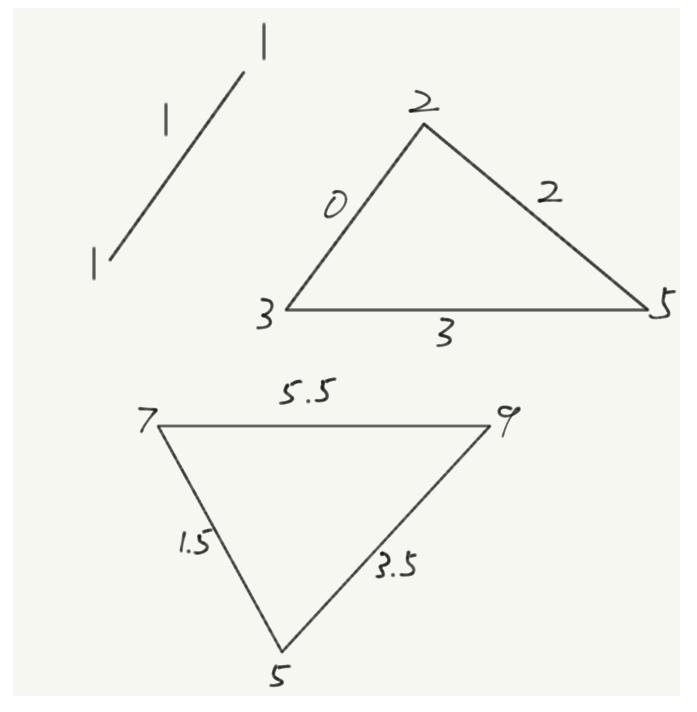
\includegraphics[scale=0.6]{10250.png}
		\caption{}
		\label{fig:1}
	\end{figure}
	(4) Since it is a weighted graph score, it is the score of a graph with real edge weights.

	\textbf{ID:517030910258}\par
	(1)(2) It is neither a graph score nor a multigtaph score because the sum of the ID is an odd number.
	(3) It is a weighted graph score, as is shown in the following figure.
	
	\begin{figure}[H]
		\centering
		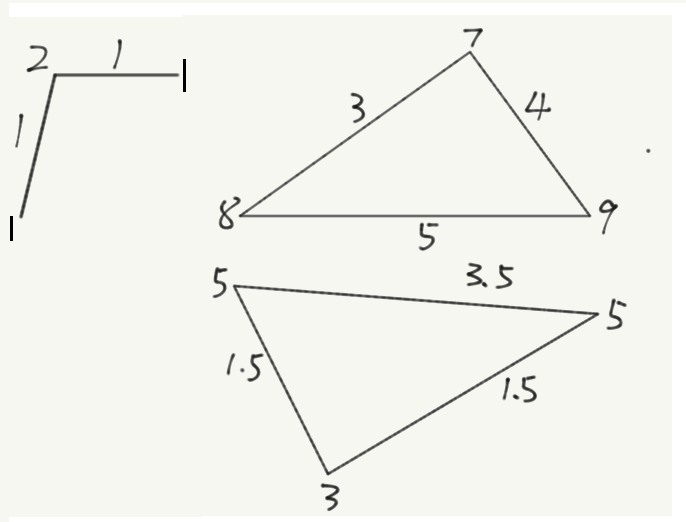
\includegraphics[scale=0.6]{10258.png}
		\caption{}
		\label{fig:2}
	\end{figure}
	(4) Since it is a weighted graph score, it is the score of a graph with real edge weights.

	\textbf{ID:517030910029}\par
	(1)(2) It is neither a graph score nor a multigtaph score because the sum of the ID is an odd number.
	(3) It is a weighted graph score, as is shown in the following figure.
	
	\begin{figure}[H]
		\centering
		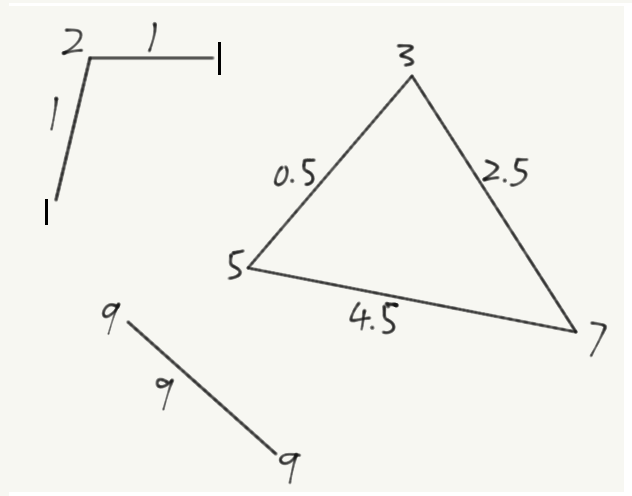
\includegraphics[scale=0.6]{10029.png}
		\caption{}
		\label{fig:3}
	\end{figure}
	(4) Since it is a weighted graph score, it is the score of a graph with real edge weights.

	\textbf{ID:517030910227}\par
	(1)(2) It is neither a graph score nor a multigtaph score because the sum of the ID is an odd number.
	(3) It is a weighted graph score, as is shown in the following figure.
	
	\begin{figure}[H]
		\centering
		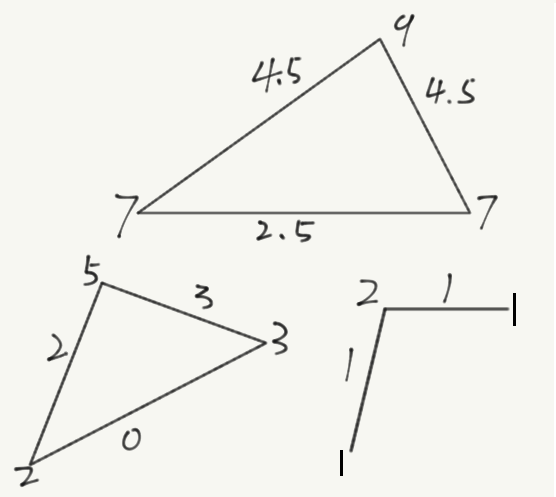
\includegraphics[scale=0.6]{10227.png}
		\caption{}
		\label{fig:4}
	\end{figure}
	(4) Since it is a weighted graph score, it is the score of a graph with real edge weights.

	\textbf{ID:517030910263}\par
	(1)(2) It is neither a graph score nor a multigtaph score because the sum of the ID is an odd number.
	(3) It is a weighted graph score, as is shown in the following figure.
	
	\begin{figure}[H]
		\centering
		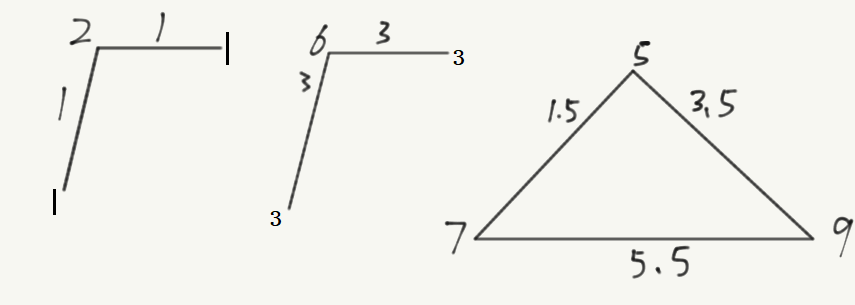
\includegraphics[scale=0.6]{10263.png}
		\caption{}
		\label{fig:5}
	\end{figure}
	(4) Since it is a weighted graph score, it is the score of a graph with real edge weights.

	\textbf{Questions}\par
	Is there a practical algorithm to tell whether two graphs are isomorphic?


\end{document}
	

